\section{Exploring the framework analytically \label{sec:explorefram}}

The chapter so far has explained the structure of the model framework. It has been noted that the units and parameters have all been kept as simple as possible and, since the model is abstract, are normalised where they can be. This section explores some of the essential mathematical relationships present in the model. This is the right location for such a discussion, as it helps set the context for the results chapter. But it is worth noting that many of the findings here were a direct result of the model framework producing results that required explanation. When the agent model produced a particular outcome, was it due to Actors acting rationally? If so, what factors were at work? The framework proposed these questions, but a full answer required a more analytic approach. As discussed in the conclusion, this is a happy synergy: the agent model helping to highlight possible lines of inquiry, and an analytic approach shedding further light on the issues.
\cmt{`As discussed in conclusion': abm and analytics bouncing off each other.}

\subsection{The effects of changing costs \label{sec:explorechangingcosts}}

The nature of basic space costs in the model is best understood by assuming only one good $g$ is produced. In this situation, utility is simply a function of the level of consumption of that one good, and it can be normalised: $U = g$. If both a Person's wage $w$ and the base cost of the good (excluding any space cost) are also normalised to one, the maximum utility is always just one.
\cmt{the one-good assumption is discussed somewhere else... where?}

From section \ref{sec:spacecost1}, the total price $P_g$ of $g$ was given as $p_g + (c \cdot d)$: the base price, delivery cost per unit distance, and the distance itself. Given the normalisations just mentioned, the question People can ask is: `what amount of $g$ can I get for my wage?' This amount, $w / P_g$, is dependent on $c$ and $d$ (assuming the base price is one). So how is `the amount I can get for my wage' affected by space? Partials for the per-unit distance cost and distance itself are functionally equivalent. Label $w / P_g$ as $Y$:

\begin{equation}
\frac{\delta Y}{\delta c} = - \frac{w\cdot d}{(1+c\cdot d)^2}
\label{eq:delcostpartial_c}
\end{equation}

\begin{equation}
\frac{\delta Y}{\delta d} = - \frac{w\cdot c}{(1+c\cdot d)^2}
\label{eq:delcostpartial_d}
\end{equation}

\begin{figure}%
\centering
\subfloat[$\frac{\delta Y}{\delta c} = - \frac{w\cdot d}{(1+c\cdot d)^2}$]
{\label{fig:partialdel1}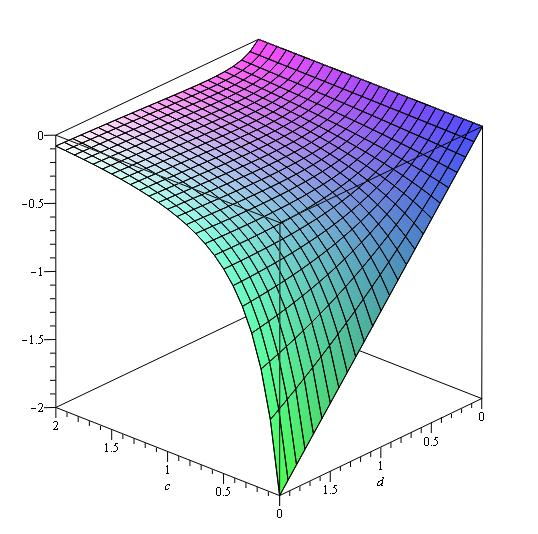
\includegraphics[width=0.4\textwidth]{ChapterFramework/figures/delCostPartial_C}}
 \hspace{0.1}
 \subfloat[$\frac{\delta Y}{\delta d} = - \frac{w\cdot c}{(1+c\cdot d)^2}$]
{\label{fig:partialdel2}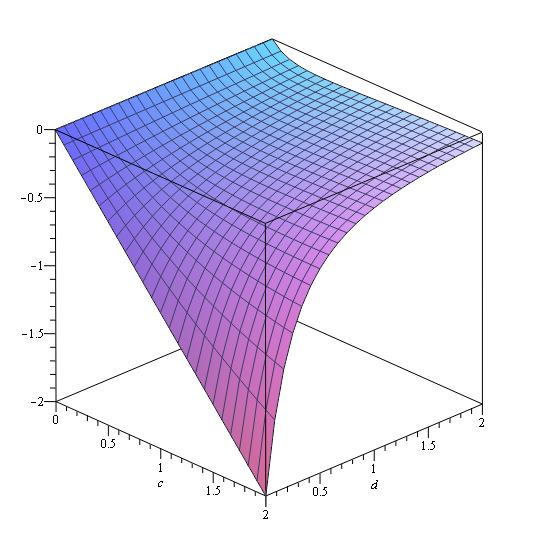
\includegraphics[width=0.4\textwidth]{ChapterFramework/figures/delCostPartial_D}}
\caption{Graphs of partial derivatives for $c$ and $d$ from $Y = w / 1 + c \cdot d$. Graphs assume $w=1$.}%
\label{fig:delcostpartials}%
\end{figure}

Allowing $w$ to be one, these are graphed in figure \ref{fig:delcostpartials}. Consider $\delta Y\delta d$ (figure \ref{fig:partialdel2}) first: how distance $d$ changes `what I can buy with my wage', holding distance cost $c$ constant. Take $c = 0$: with no distance cost, distance itself does not change what I can buy. As $c$ increases, however, $d$ has a larger impact earlier on, and the dropoff is steeper as the delivery cost goes up. So, where $c = 2$ and $d = 2$, there's much less of a drop in what I can buy with my wage if I change either of them.
 	 	 
$\delta Y\delta d$ (figure \ref{fig:partialdel1}) is structurally exactly the same, but highlights a slightly different point. 

What it's saying: look at where d is 2. What's happening with c? Well, "the amount I can buy with my wage" decreases much more rapidly for changes in smaller quantities of delivery cost than larger. 
OK: so that should all explain why we get this:
That's with density costs set to zero. Interestingly the shape wasn't so different with density costs present - oh, that would be because people can't move and their location is evenly spread: the cost will be the same for all of them, pretty much.
OK, just spent some time wiggling the delivery cost in the vis and I think I get it now - particularly for dy/dc. The changes are much more rapid for the those further away as dc increase. The change - proportional to what is much smaller utility - as they become high is much, much smaller.
So if we're imagining a Glaeser-like situation where transport costs are very low, that's interesting: it's possibly saying, changes in transport costs when they're low will have a larger impact than shifting between already-high transport cost-areas. 
I think partial diff might be magic. 
Except that doesn't account for transport costs as a \% of base price. I think (though am checking below) it's going to mean: changes in transport costs in low-transport cost situations will affect low value density cost goods more than high value. Which is intuitive enough, if you've managed to hold onto all the bits of that to the end of this sentence.
